 \documentclass{openetcs_report}
% Use the option "nocc" if the document is not licensed under Creative Commons
%\documentclass[nocc]{template/openetcs_article}
\usepackage{todonotes}
\usepackage{appendix}
\usepackage{lipsum,url}
\usepackage{pdfpages}
%\usepackage{bibtopic} % Multibib
\usepackage{booktabs}
\usepackage[hidelinks]{hyperref}
\usepackage[section,                 % add the glossary to the table of content 
            description,             % acronyms have a user-supplied description,
            style=superheaderborder, % table style
            nonumberlist             % no page number
]{glossaries}
%===========================
% Graphicpath
%===========================
\graphicspath{{./template/}{.}{./images/}}

%===========================
% Abbreviation file
%===========================
\renewcommand*{\glossaryname}{List of Terms}
\makeglossaries
\loadglsentries{wp7_glossary} 
%===========================
%===========================
% Todo note margin
%===========================
\setlength{\marginparwidth}{7em}
%===========================

\begin{document}
\frontmatter
\project{openETCS}

%Please do not change anything above this line
%============================
% The document metadata is defined below

%assign a report number here
\reportnum{OETCS/WP7/O7.3.2}

%define your workpackage here
\wp{Work-Package 3: ``Tool chain''}

%set a title here
\title{Tool chain Development Plan}

%set a subtitle here
\subtitle{Description of the tool chain}

%set the date of the report here
\date{August 2013}

%define a list of authors and their affiliation here

\author{Cecile Braunstein \and Jan Peleska}

\affiliation{University Bremen}



% define the coverart
\coverart[width=350pt]{openETCS_EUPL}

%define the type of report
\reporttype{Tool chain Architecture}


\begin{abstract}
%define an abstract here
This document defines the tool chain architecture : the links between
the tools and the interoperability mechanism implemented.

The present tool chain will propose some alternative path to give more
flexibility with the chosen tools.
\end{abstract}

%=============================
%Do not change the next three lines
\maketitle
\tableofcontents
\listoffiguresandtables

\newpage
%=============================

% The actual document starts below this line
%=============================
%Start here
%=============================
% Document Managment
%=============================
\chapter{Document Information}
\begin{tabular}{|p{4.4cm}|p{8.7cm}|}
\hline
\multicolumn{2}{|c|}{Document information} \\
\hline
Work Package &  WP7  \\
Deliverable ID or doc. ref. & O7.3.2\\
\hline
Document title & Tool chain architecture \\
Document version & 00.00 \\
Document authors (org.)  & Cécile Braunstein  (Uni.Bremen)  \\
& Jan Peleska (Uni. Bremen)\\
\hline
\end{tabular}

\begin{tabular}{|p{4.4cm}|p{8.7cm}|}
\hline
\multicolumn{2}{|c|}{Review information} \\
\hline
Last version reviewed &  \\
\hline
Main reviewers & \\
\hline
\end{tabular}

\begin{tabular}{|p{2.2cm}|p{4cm}|p{4cm}|p{2cm}|}
\hline
\multicolumn{4}{|c|}{Approbation} \\
\hline
  &  Name & Role & Date   \\
\hline  
Written by    &  Cécile Braunstein & WP7-T7.3 Sub-Task  & \\
& Jan Peleska & Leaders&\\
\hline
Approved by & &  & \\
\hline
\end{tabular}

\begin{tabular}{|p{2.2cm}|p{2cm}|p{3cm}|p{5cm}|}
\hline
\multicolumn{4}{|c|}{Document evolution} \\
\hline
Version &  Date & Author(s) & Justification  \\
\hline  
00.00 & 25.07.2013 & C. Braunstein  &  Document creation  \\
\hline  
\end{tabular}
\newpage
%==========================================


%------ List of terms and definition ----------------
\printglossary
%==========================================
\mainmatter
%----------------------
\chapter{Introduction and Motivation}
\todo[color=green!40,noline]{Chap resp. CB/JP}


%-----------------------
\section{Motivation}
%-----------------------

%-----------------------
\section{Scope of the document}
%-----------------------

%----------------------
 \section{Reference documents}
%----------------------- 
\begingroup
%\renewcommand{\section}[2]{}%
\renewcommand{\chapter}[2]{}% for other classes
  \bibliographystyle{plain}
  \bibliography{wp7_bibliography}
\endgroup
%%% Local Variables: 
%%% mode: latex
%%% TeX-master: WP7-Toolchain_architecture"
%%% End: 



%----------------------
\chapter{OpenETCS Tool chain Presentation}
%----------------------
\label{chap:toolchaindef}
\todo[color=green!40,noline]{Chap resp. CB/JP}

%----------------------------------------------------
\section{The OpenETCS tool chain}
%----------------------------------------------------
\subsection{Definition}
%----------------------------------------------------
The tool chain provides the tool support and the development process
to provide a formalized specification of \gls{SRS} and an executable
code of the \gls{OBU}.


The tool chain is composed by two kind of tools :
\begin{enumerate}
\item {\it Development tools}: those used along the phases of the software
  development process (Requirement engineering, modeling ...).
\item {\it Management tools}:  those used transversely during the
  complete development process (version management, requirements
  traceability ...).
\end{enumerate}
These tools are called vertical and horizontal tools in
\cite{wasserman_tool_1990}. 
Figure \ref{fig:toolchain} shows the idea of the complete tool chain
integration.

\begin{figure}[htbp]
\centering
  \includegraphics[width=.5\textwidth]{images/toolchain_archi-dev}
  \caption{The OpenETCS tool chain}
  \label{fig:toolchain}
\end{figure}

In the next chapters  we will give more details on the
data integration between the development tools by defining the inputs
and outputs artifact of each tools. This document describes the
interface between the tool chain activities.
The interoperability mechanism will be defined in a separate
document. However, the first version of the tool chain will implement a
file-based data exchange.
 
It has been decided (see \cite{D7.1}) that the tool platform hosting
the tool chain is Eclipse with the Eclipse modeling framework
(\gls{EMF}).  This implies that the tool chain will be a set of
Eclipse plug-ins. It also implies that we can rely on already
available plug-in and features for the versioning, the project
management or the build system.  The use of EMF will also assist the
software development, by providing a meta model and an \gls{API} for
manipulating EMF components.


%----------------------------------------------------
\subsection{The SysML Model}
%----------------------------------------------------
A SysML model of the tool shown figure \ref{fig:overview} . It
allows us to have a formal representation of the tool chain and
help to model precisely the different interaction between the
development tools as well as the management tools.  The SysML model
may be also seen as a guideline for integrated new tool: each new tool
should be fully described and comply to the defined interfaces.
Moreover following the idea of Slotosch \cite{slotosch_iso_2012} the
model will be the basis to the qualification analysis \cite{D7.3}.

\begin{figure}[htbp]
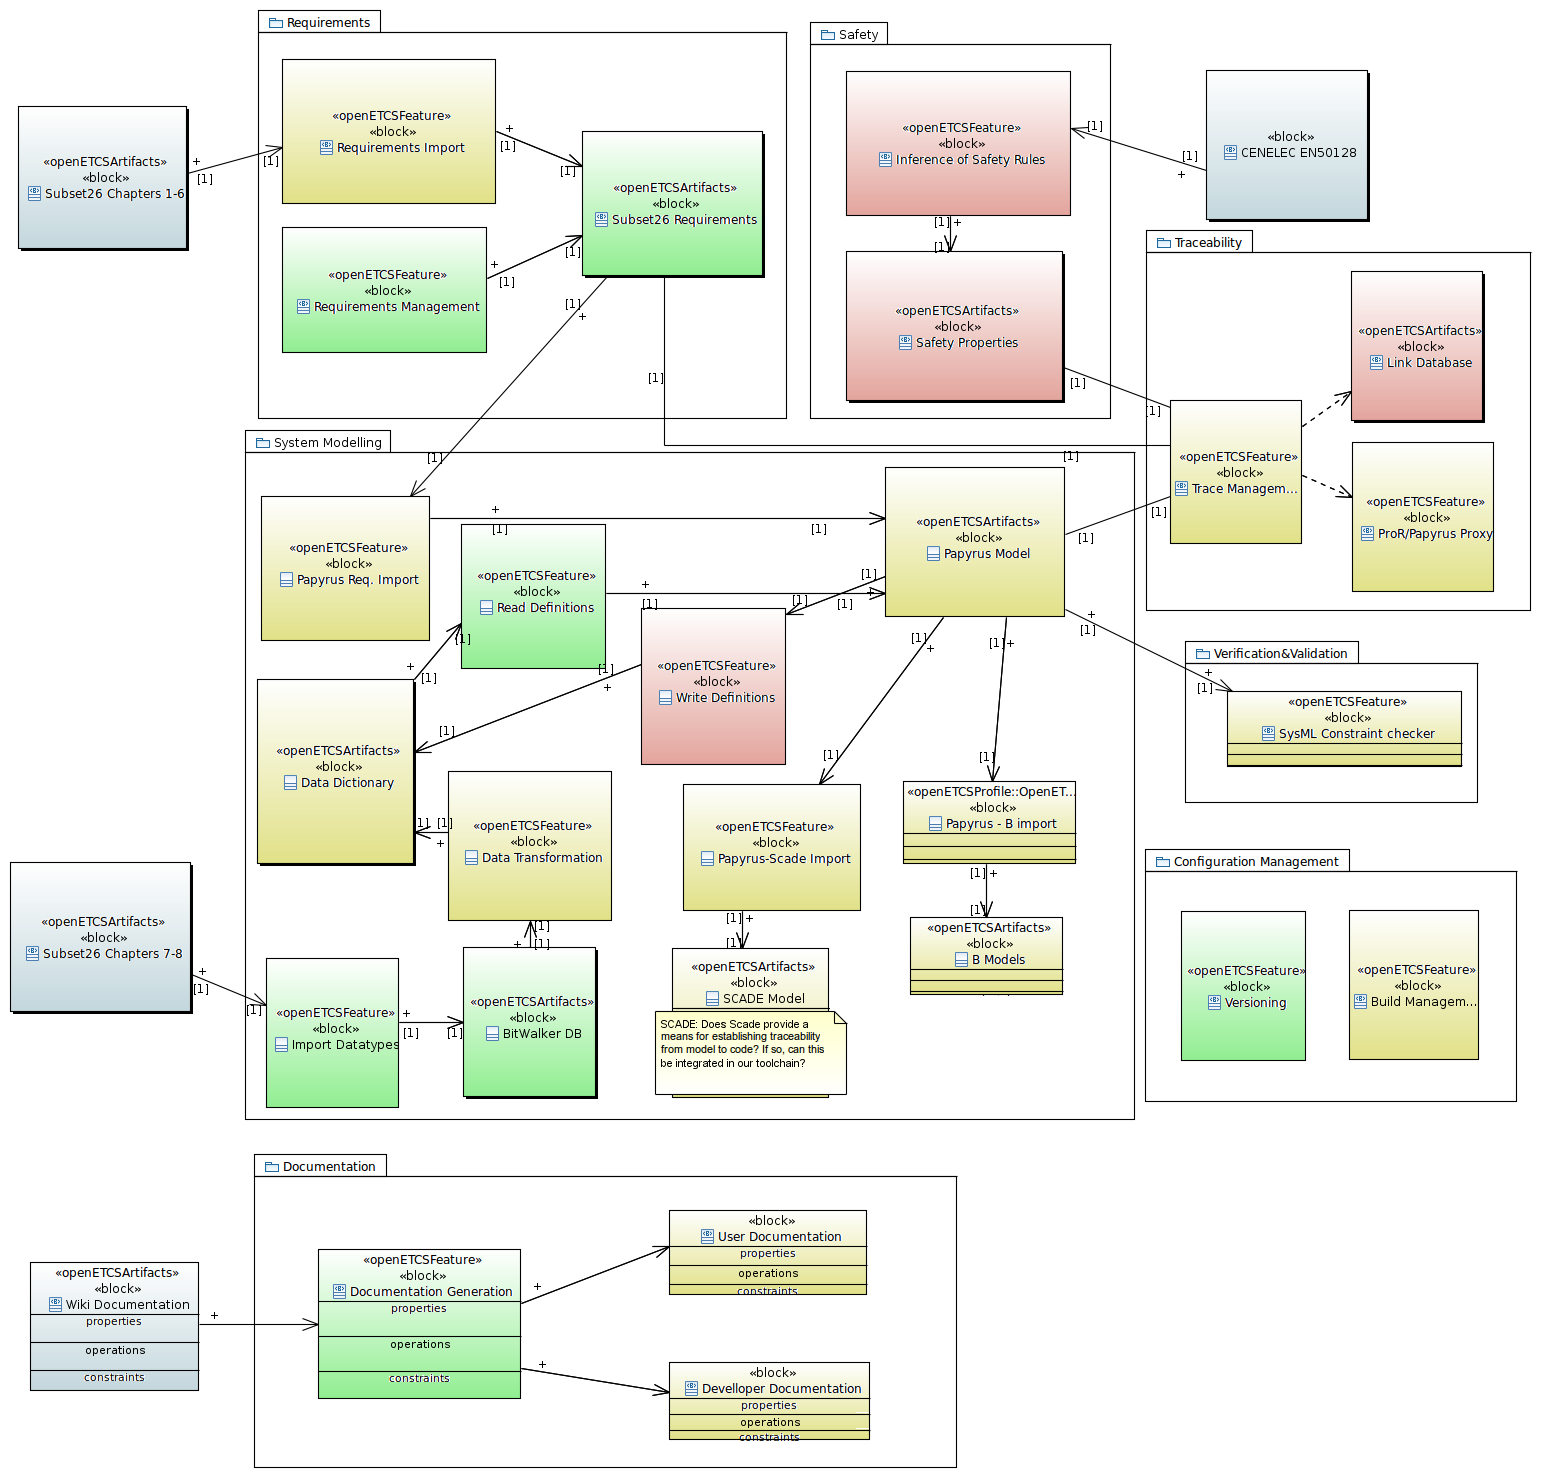
\includegraphics[width= \textwidth]{images/ToolChainmodel.png}
\caption{\label{fig:overview}OpenETCS tool chain Status Overview}
\end{figure}
\todo[inline]{Check if the overview is up-to-date and complient with
  the real implementation}

The requirements of WP2 \cite{baro_requirements_2013} as well as our
intern requirements (Appendixes \ref{app:wp2req} and \ref{app:WP7Req})
will be included in the SysML model. Each tools and their connections
should then also comply to the requirements list.


%----------------------------------------------------
\subsection{The OpenETCS lifecycle}
%----------------------------------------------------
\todo[inline]{Insert the tool chain lifecycle definition from WP1}
%----------------------------------------------------
\section{OpenETCS \gls{EVC} lifecycle}
%----------------------------------------------------
The openETCS lifecycle has been defined in 
 \cite{D2.3} as  presented figure \ref{fig:openETCSProcess}.
\begin{figure}[htbp]
  \centering
  \includegraphics[width= \textwidth]{images/ProcessOpenETCS}
  \caption{openETCS Process (rough view)}
  \label{fig:openETCSProcess}
\end{figure}

The lifecycle defined all the different steps needed to produce a
\gls{EVC} certifiable SIL4. However in order to define a tool chain we
need to define the lifecycle by means of activities
(Fig. \ref{fig:openETCSActivities}). Each activities may be achieved by
one or more tools in the tool chain. 

The next chapters will define the limits of each activities, we will
show what should be consumed and produced by each activities. 
\begin{figure}[htbp]
  \centering
  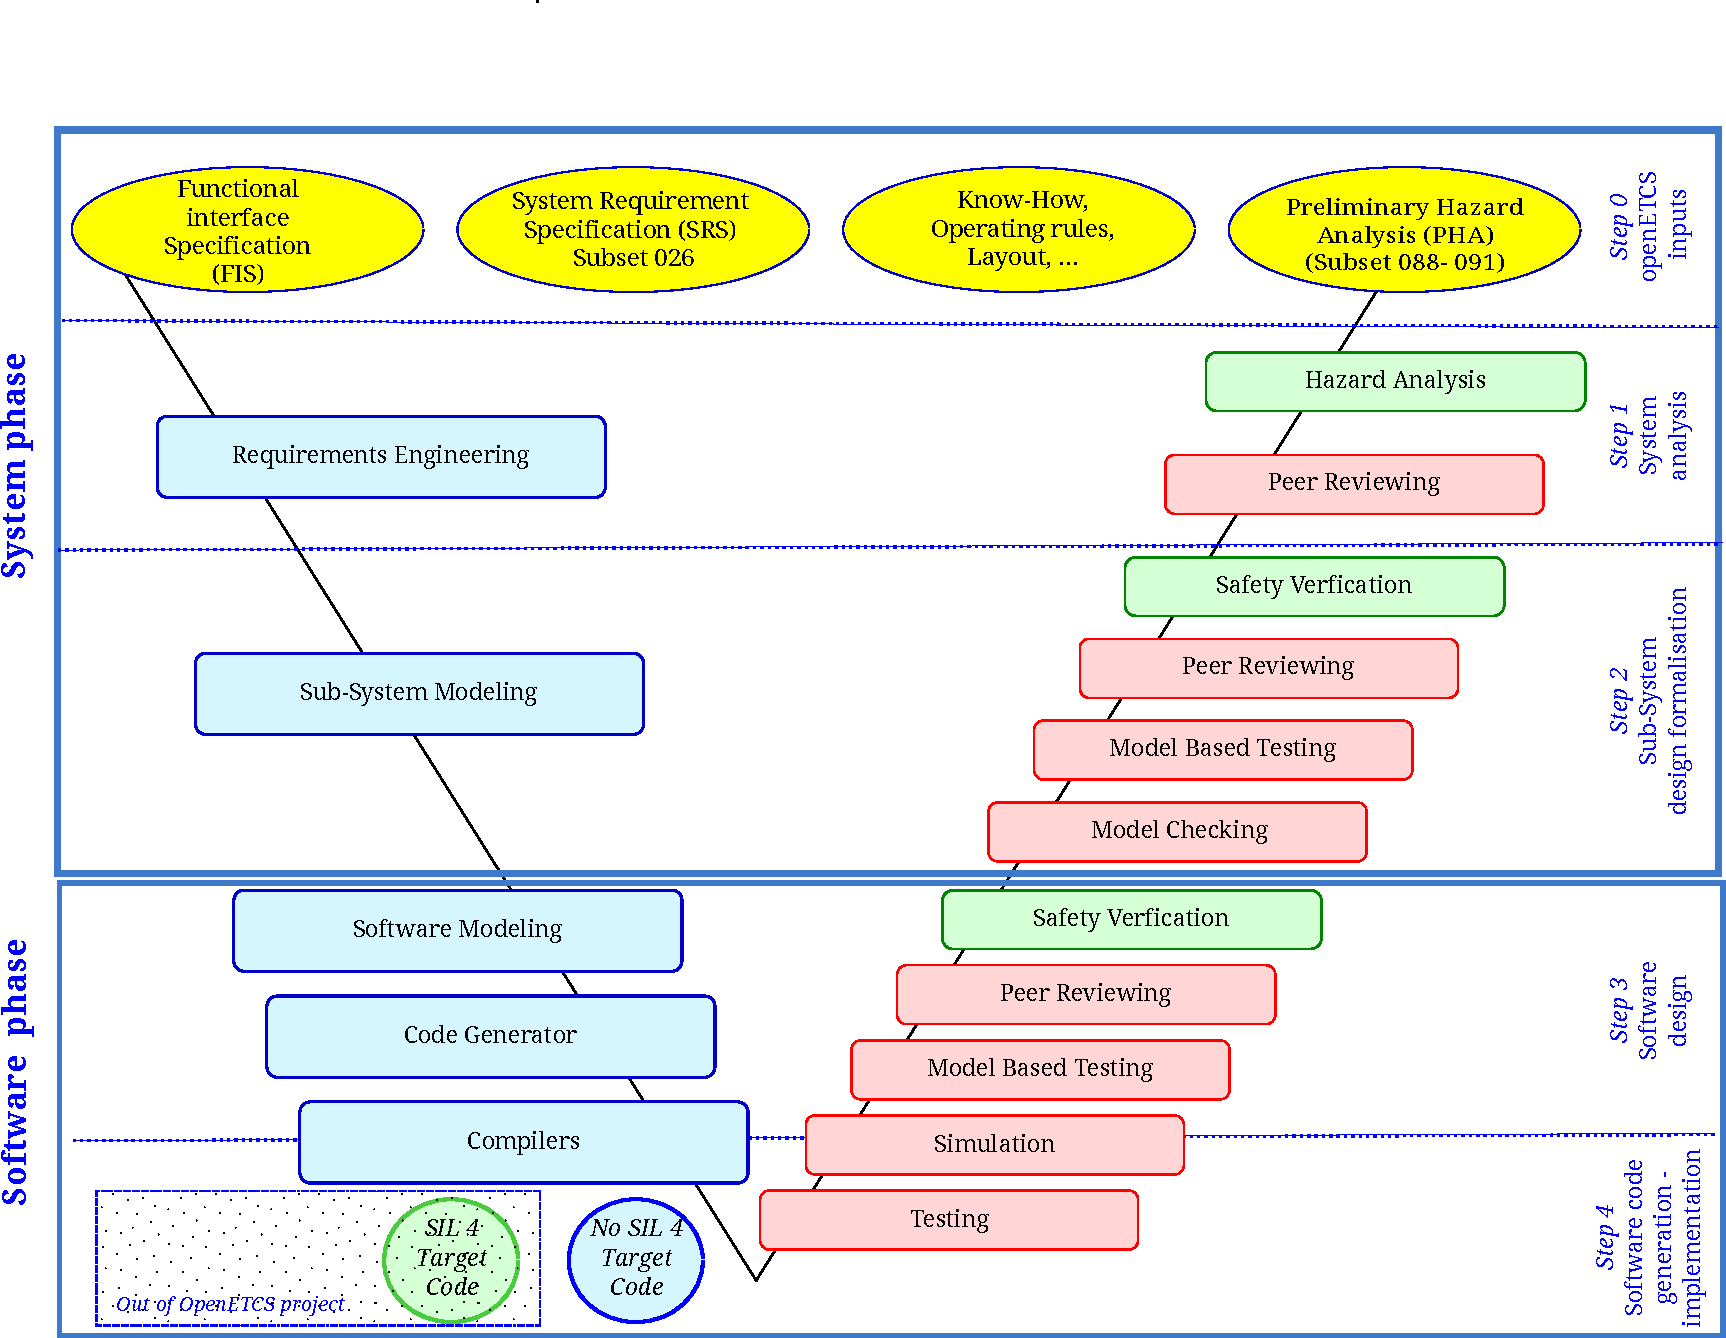
\includegraphics[width=\textwidth]{images/WholeProcess_Activities}
  \caption{openETCS Process Tool chain activities}
  \label{fig:openETCSActivities}
\end{figure}

\todo[inline]{add description of each activities}

%----------------------------------------------------
\section{Management tools}
%----------------------------------------------------
\todo[inline] {add the list of the management tools and a description}
\begin{itemize}
\item Version Management\\
Version management of the artifacts and the openETCS glue code 
\item Tool version Management \\
Keep track of the compatible and status version of each tools. 
\item Collaborative work
\item Project  Management
\item Build system
\item Non regression test
\item Configuration Manger to manage modification and change in tools
\end{itemize}



%%% Local Variables: 
%%% mode: latex
%%% TeX-master: "WP7-Toolchain_architecture"
%%% End: 


%----------------------
\chapter{OpenETCS Requirement Engineering}
%----------------------
\label{chap:reqhandling}
\todo[color=green!40,noline]{Chap resp. ??}

\section{Activities purpose}
Requirement engineering is the starting point of the modeling
activities. It is the basis for describing how  all the actors and
tools may interact to produce the desired system. 

In OpenETCS the specification describing the requirement comes from
three document, two of them related to the \gls{ERTMS}
\cite{unisig_subset-026_2012,unisig_subset-034-_2012}, the third one
to the know-how of the operators and the different actors of the
design process. The translation into a requirement database in
computer readable format remains a manual task.

Figure \ref{fig:reqHand} presents different tools alternative to
realize the requirement management activities within our tool
chain. The activity may be achieved by combining some of these tools
to get the best of each. For example one can start by collecting the
requirements in a csv format and then add the dependency with ProR or
Papyrus.
\begin{figure}[htbp]
  \centering
  \includegraphics[width=\textwidth]{images/Req_Hand}
  \caption{Requirement Engineering}
  \label{fig:reqHand}
\end{figure}


\todo[inline]{Tools description or reference to their description}

\section{Input/Output artifacts}
\todo[inline]{Take a decision to the interface or exhibits the compatibility
  between the format and how it may be achieved}

%%% Local Variables: 
%%% mode: latex
%%% TeX-master: "WP7-Toolchain_architecture"
%%% End: 


%----------------------
\chapter{OpenETCS Sub-System Modeling}
%----------------------
\label{chap:sysphase}
\todo[color=green!40,noline]{Chap resp. ??}

It has been decided \cite{} to use SysML as a modeling language and
papyrus as modeling tool. \todo{add references}

The use of SysML is restricted to the following :
\begin{itemize}
\item Requirements:
  \begin{itemize}
    \item Requirement Diagram
    \item Requirement relationships : {\tt verify}/{\tt satisfy}/{\tt
        trace}
  \end{itemize}
\item Structures:
  \begin{itemize}
    \item Block Diagram
    \item Internal Block Diagram
    \item Ports
  \end{itemize}
\item Behaviors:
  \begin{itemize}
  \item State machines
  \item Activity diagram (optional)
  \end{itemize}
\end{itemize}

All tool  should be able to understand and to produce the same SysML format.

\subsection{Input/Output artifacts}
%%% Local Variables: 
%%% mode: latex
%%% TeX-master: "toolchain_archi"
%%% End: 


%----------------------
\chapter{OpenETCS  Software Modeling}
%----------------------
\label{chap:softphase}
\todo[color=green!40,noline]{Chap resp. ??}

\begin{figure}[htb]
  \centering
  \includegraphics[width=\textwidth]{images/modeling_phase2}
  \caption{Software phase description}
  \label{fig:softPhase}
\end{figure}

\subsection{Input/Output artifacts}
%%% Local Variables: 
%%% mode: latex
%%% TeX-master: "toolchain_archi"
%%% End: 


%----------------------
\chapter{V\&V tools}
%----------------------
\label{chap:VnV}
\todo[color=green!40,noline]{Chap resp. ??}


%----------------------
\chapter{Interoperability specification}
%----------------------
\label{chap:interope}
\todo[color=green!40,noline]{Chap resp. ??}

To make the tool chain flexible, easy to maintained etc ... We need to
define the interface between the tools in a loosely way. The interoperability
mechanism should assist the flexibility as well as give some guidance
to integrate new tools along the tool chain development. 

We propose that for each tool chain activities the WP7 will agree on a
common input/output format. This will help to link the activities
altogether and ease the tools update or change.
It keeps the tools independent.

That implies to have an open interoperability specification.
The interoperability mechanism can be decomposed in different
concept.
\begin{itemize}
\item Architecture: what are the principles of the interoperability
  mechanism all tools agree on (e.g. RESTful architecture)
\item Communication : the communication protocol and data exchange
  format (e.g. XML)
\item Syntax: the structure of information represented in a common
  data format. What tools need to parse and interpret information
  (e.g. RDF)
\item Semantic layer : Basic semantic to make the tools understand
  each others. (e.g. Meta model EMF)
\end{itemize}

The OSLC project proposes a set of standard interface to link  the
different lifecycle activities together. The idea is to have a common
core protocol and architecture and then for each activities a
domain specific interface. All activities do not necessarily share the
same interest for the same data. Some part of the interfaces are
already covered, others still need to be specify. The amount of needed
work to comply to this specification should be quantified and a
decision of whether or not OpenETCS join the OSLC project should be
made.

During the tool chain development we need to maybe go step by step and
start with exchange by file and then add more restful architecture.
At each development step each tool should conform to the defined
interface.



%%% Local Variables: 
%%% mode: latex
%%% TeX-master: "WP7-Toolchain_architecture"
%%% End: 


%----------------------
\chapter{Integration in the tool platform}
%----------------------
\label{chap:integration}
\todo[color=green!40,noline]{Chap resp. ??}

\todo[inline]{Fill for each plugin}

\begin{tabular}{|lp{0.7\textwidth}|}
\hline
\multicolumn{2}{|c|}{\bf Feature/plug-in Name}\\
\bf Version&\\
\bf Activities covered&\\
\bf Documentation link&\\
\bf Tutorial links&\\
\bf Short Description&\\
\bf Unit tests references&\\
\bf Covered Requirements&\\
\hline
\end{tabular}





%%% Local Variables: 
%%% mode: latex
%%% TeX-master: "WP7-Toolchain_architecture"
%%% End: 




\appendix

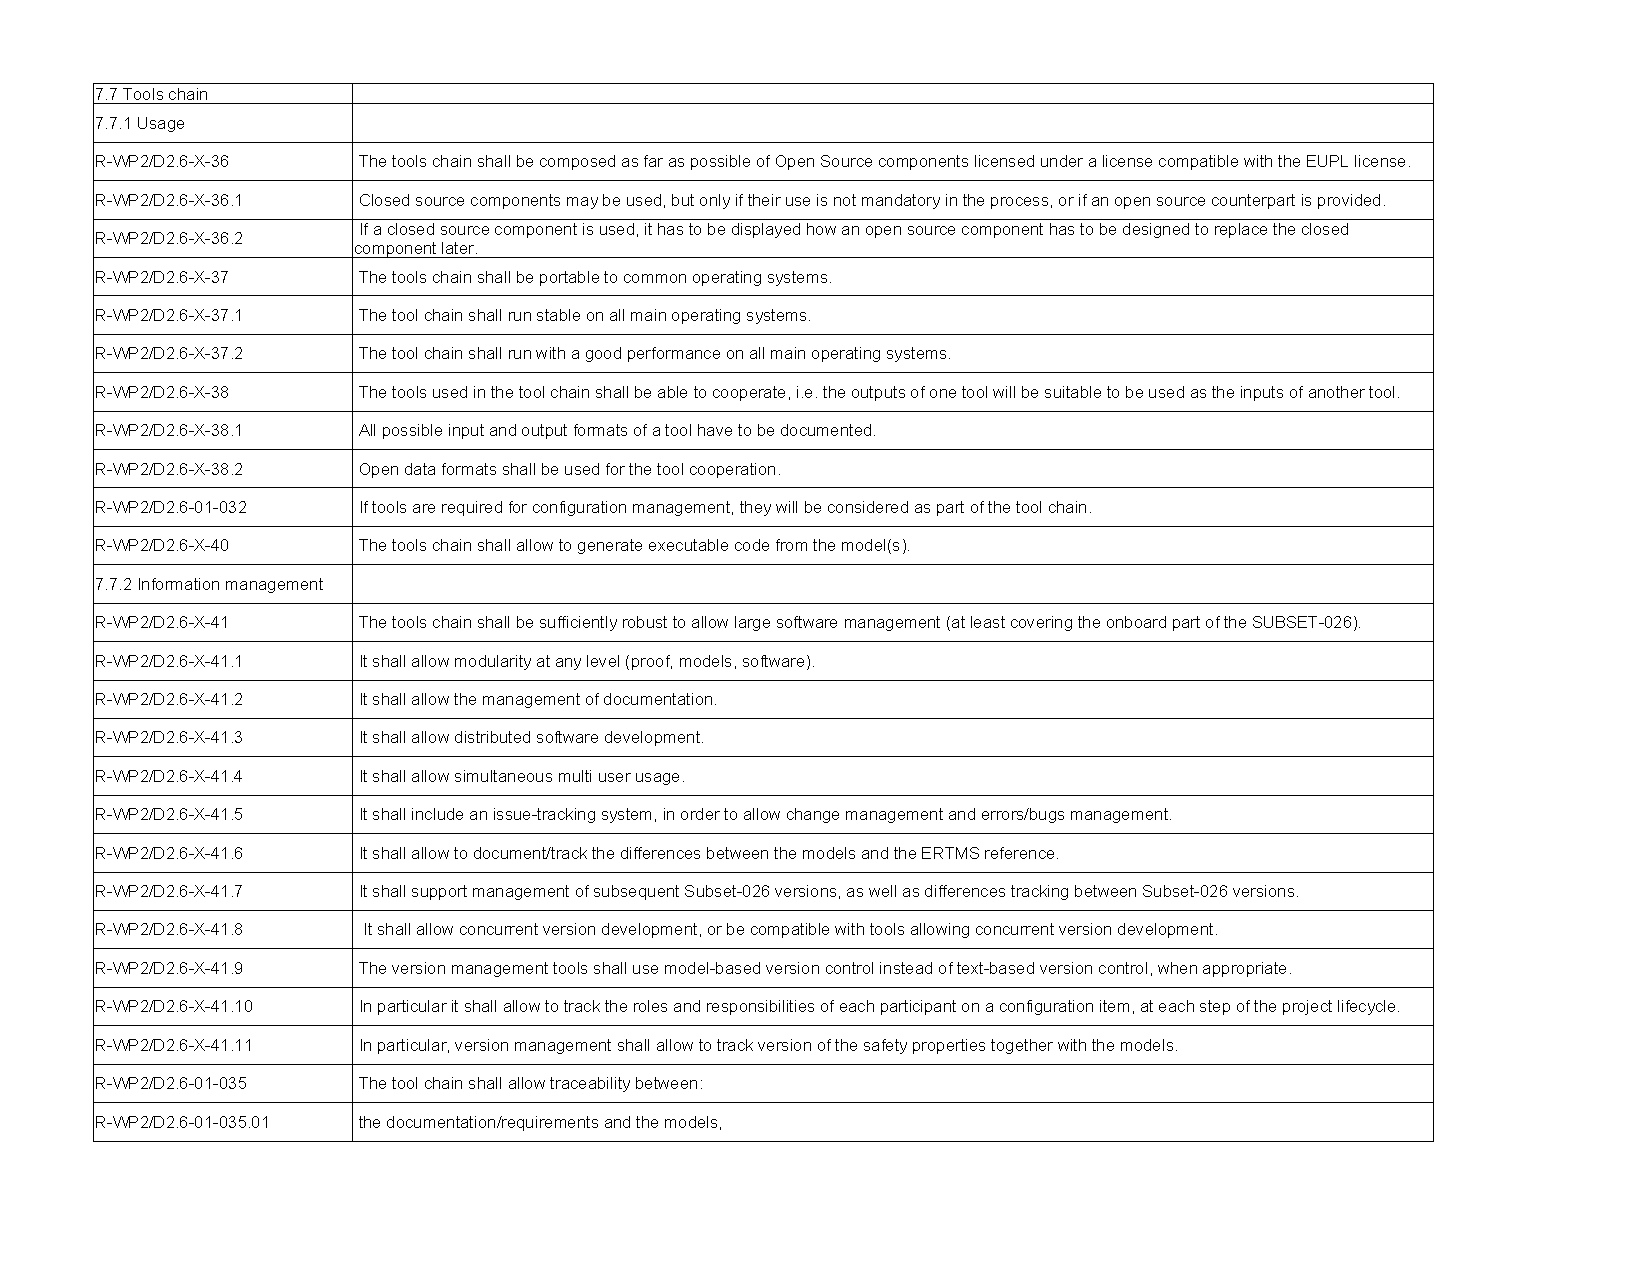
\includepdf[pages={1},landscape=true,pagecommand=\chapter{WP2
  requirements}\label{app:wp2req}]{images/req_D2_6.pdf}

\includepdf[pages={2},landscape=true,pagecommand={}]{images/req_D2_6.pdf}

\chapter{WP7-specific requirements}
\label{app:WP7Req}

%% Requirements.


\newcounter{reqnum}
\setcounter{reqnum}{0}
\newcounter{subreqnum}
\newcounter{subsubreqnum}
\newlength{\partopbuf}
\newlength{\topbuf}

% Automated numbering versions of the macros
\newcommand{\req}[1]{\addtocounter{reqnum}{1} \setcounter{subreqnum}{0}
	\begin{description}\item[{\small\reqt-X-\thereqnum}] #1\end{description}
}

\newcommand{\subreq}[1]{
	\addtocounter{subreqnum}{1} \setcounter{subsubreqnum}{0}
	\addtolength{\leftmargini}{1cm}
	\begin{description}
	\item[\hspace{0.5cm}{\small\reqt-X-\thereqnum.\thesubreqnum}] #1
	\end{description}
	\addtolength{\leftmargini}{-1cm}
}

\newcommand{\subsubreq}[1]{
	\addtocounter{subsubreqnum}{1}
	\addtolength{\leftmargini}{2cm}
	\begin{description}
	\item[\hspace{1cm}{\small\reqt-X-\thereqnum.\thesubreqnum.\thesubsubreqnum}] #1
	\end{description}
	\addtolength{\leftmargini}{-2cm}
}

% Fixed version of the commands
\newcommand{\reqfixed}[3]{\addtocounter{reqnum}{1} \setcounter{subreqnum}{0}
	\begin{description}\item[{\small\reqt-#1-#2}] #3\end{description}
}

\newcommand{\subreqfixed}[4]{
	\addtocounter{subreqnum}{1} \setcounter{subsubreqnum}{0}
	\addtolength{\leftmargini}{1cm}
	\begin{description}
	\item[\hspace{0.5cm}{\small\reqt-#1-#2.#3}] #4
	\end{description}
	\addtolength{\leftmargini}{-1cm}	
}

\newcommand{\subsubreqfixed}[5]{
	\addtocounter{subsubreqnum}{1}
	\addtolength{\leftmargini}{2cm}
	\begin{description}
	\item[\hspace{1cm}{\small\reqt-#1-#2.#3.#4}] #5
	\end{description}
	\addtolength{\leftmargini}{-2cm}	
}

% Citation of the requirement

% Citation of the reference (for markup purpose)
%\newcommand{\refreq}[1]{\textbf{#1}}

% Citation of the reference and text (for markup purpose)
% The purpose of this is to automatically replace the placeholder by the 
% full text. \fullrefreq{R-xxx}{} or \fullrefreq{R-xxx}{blabla} 
% will be replaced by \fullrefreq{R-xxx}{text of the R-xxx requirement} 
%\newcommand{\fullrefreq}[2]{\textbf{#1}: \textrm{#2}}


\def\reqt{R-WP7/T7.3}
\req{The tool chain shall include support for the following graphical user interface facilities:}
\subreq{model syntax highlighting and auto-completion, for the parts of the model that are text-based}
\subreq{graphical representation of Subset-026 braking curves}

\subreq{tree-based display of model elements}
\subreq{model animation and debugging}
\subreq{perspective management: offer in a single graphical user interface several interconnected views for SRS, model and tests.}
\req{The tool chain shall provide the following reporting facilities:}
\subreq{detailed implementation metrics}
\subreq{detailed traceability reports}
\subreq{detailed model errors and warnings list}

\todo{to be continued}

%%% Local Variables: 
%%% mode: latex
%%% TeX-master: "toolchain_archi"
%%% End: 


%===================================================
%Do NOT change anything below this line

\end{document}
